\documentclass{article}
\usepackage[utf8]{inputenc}
\usepackage[german]{babel}
\usepackage{underscore}
\usepackage{xcolor}
\usepackage{listings}
\usepackage{graphicx}
\usepackage{hyperref}

\usepackage{xparse}

\NewDocumentCommand{\codeword}{v}{%
\texttt{\textcolor{blue}{#1}}%
}

\lstset{language=VHDL,keywordstyle={\bfseries \color{purple}}}

\title{ERA-Projekt 2 - Spezifikation}
\author{Adrian Regenfuß, Till Müller, Korbinian Stein}
\begin{document}
\maketitle
\section{Organisatorisches}
  \subsection{Aufgabenverteilung}
    Projektleitung: Till Müller\\
    Verantwortlicher Vortrag: Adrian Regenfuß\\
    Verantwortlicher Dokumentation: Korbinian Stein
  \subsection{Zeitplanung}

  	\begin{tabular}{r | l}
  		\textbf{Zeitpunkt}&\textbf{Aufgabe}\\
  		20.04.&Grundsätzliche Ideen\\
  		27.04.&Definition und Formulierung der zwei Ansätze\\
  		13.05.&\emph{Fertigstellung Spezifikation}\\
  		18.05.&Grobe Fertigstellung der Rahmenstruktur (Makefile, GTKWave, GHDL)\\
  		01.06.&Erste Ansätze in VHDL\\
  		08.06.&Ausarbeitung der Testumgebung\\
  		15.06.&Fertigstellung des Bausteins und der Tests\\
  		17.06.&\emph{Fertigstellung Implementierung}\\
  		29.06.&Erste Zusammenstellung der zu dokumentierenden Informationen\\
  		13.07.&Ausformulierung der Dokumentation\\
  		20.07.&Zusammentragen der Protokolle\\
  		23.07.&Vorträge fertiggestellt\\
  		28.07.&\emph{Fertigstellung Ausarbeitung}\\
  	\end{tabular}

\section{Über die Aufgabe}
  Eingabe: Parallele Daten vom Speicher, Taktrate, Datensignal vom Speicher\\
  Ausgabe: Serielle Daten nach gegebenem Protokoll (siehe Abb. \ref{img:Protokoll})

\section{Ist/Soll Analyse}
  \subsection{Ist}
    Der zu implementierende Baustein Parallel-Seriell-Konverter (im Nachfolgenden PS), hat 3 Eingänge und 2 Ausgänge. Die Eingänge bestehen aus \codeword{clk : std_logic} für den Takt, \codeword{P : std_logic_vector(15 downto 0)} für den parallelen Eingang und \codeword{S : std_logic} das dem PS signalisiert, dass gerade keine Daten gelesen werden dürfen.
    Die Ausgänge bestehen aus \codeword{LO : std_logic} für das seriell anzulegende Signal an die Lampensteuerung, sowie \codeword{SO : std_logic} für das an die Strangsteuerung seriell anzulegende Signal.
    Wir gehen davon aus, dass das Signal \codeword{P} für den gesamten Zeitraum der Übertragungszyklen anliegt.

  \subsection{Soll}
    Der PS agiert immer innerhalb von Abschnitten zweier Übertragungszyklen. Diese sind jeweils 16 Takte lang, somit besteht ein voller Zyklus aus 32 Takten.
    Die Übertragung der Daten beginnt mit dem ersten \codeword{rising_edge} der \codeword{clk}, vorausgesetzt \codeword{S != HIGH}, also die Speichersperre ist nicht aktiv.
    Zuerst wird die Strangsteuerung angesteuert, dann die Lampensteuerung, beide folgen untenstehendem Protokoll.
    Die Daten \codeword{D0}-\codeword{D7} werden für die Strangsteuerung aus \codeword{P0}-\codeword{P7} gewonnen, und für die Lampensteuerung aus \codeword{P8}-\codeword{P15}.

    Solange \codeword{S} nicht \codeword{HIGH} wird, wird der Gesamtzyklus der Ausführung der zwei Zyklen mit den selben Bedingungen wiederholt.
    Falls während der Ausgabe das Signal \codeword{S} für die Speichersperre aktiv werden sollte, wird die Ausgabe weitergeführt (um einen undefinierten Zustand der restlichen Komponenten zu vermeiden) und der Baustein im Anschluss auf den Ausgangszustand zurückgesetzt.

    Das Ausgabeprotokoll (siehe Abbildung \ref{img:Protokoll}) für einen Übertragungszyklus, soll wie folgt umgesetzt sein:\\
    \begin{tabular}{l | l}
      \hline
      Takt  & Anliegende Signale \\
      \hline
      $0-1$ & START Teil 1: \codeword{HIGH} \\
      $2-3$ & START Teil 2: \codeword{LOW} \\
      $4-11$ & Daten \codeword{D0}-\codeword{D7}\\
      $12-13$ & STOP Teil 1: \codeword{LOW} \\
      $14-15$ & STOP Teil 2: \codeword{HIGH} \\
    \end{tabular}\\
    Während des ersten Zyklus für die Strangsteuerung wird das Datum \codeword{D0} von dieser ignoriert, also wird das in Takt 4 gesendete Signal weder gesondert verarbeitet noch beachtet.
    Da dieses aber im Speicher vorhanden ist und somit auch in \codeword{P} mitübertragen wird, muss keine Fallunterscheidung zwischen Strangsteuerung und Lampensteuerung stattfinden weil die Protokolle im übrigen identisch sind.

    \begin{figure}
      \centering
      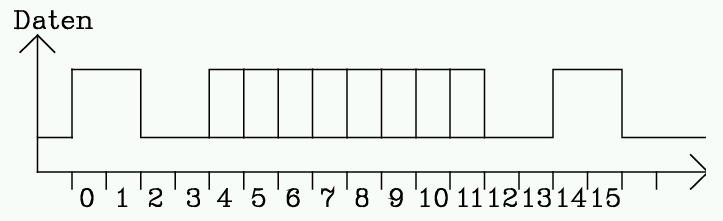
\includegraphics[width=0.8\textwidth]{protokoll.png}
      \caption{Protokoll der seriellen Ausgabe}
      \label{img:Protokoll}
    \end{figure}

    Die nach Abschnitt \ref{sec:Tests} erstellten Tests sollten ohne Probleme ausführbar sein.
    Der Baustein sollte des Weiteren auch nach zu erwartenden fehlerhaften Eingaben keine größeren Fehler auslösen und keine undefinierte Zustände annehmen.


\section{Lösungsansatz 1 \\ Lösung mittels purer \emph{State-Machine}}
  \subsection{Grundidee}
    Diese Lösung soll einen Zähler \codeword{counter} verwenden, der den aktuellen Status beinhaltet, und die Daten in einem internen Signal \codeword{data} zwischenspeichern. Dieser Zähler hat den Wertebereich $0 \leq counter \leq 31$ und den Startwert $0$.
    Mithilfe des Zählers kann festgestellt werden, in welcher Phase der Ausgabe sich der Baustein befindet, dieser wird nach jedem Takt inkrementiert.
    Nach zwei Übertragungszyklen wird der Zähler wieder auf $0$ gesetzt und die Übertragung wird weitergeführt.
    Der Gesamtzyklus beginnt abhängig von der Speichersperre erst, wenn diese nicht aktiv ist.
  \subsection{Umsetzung des Zählers}
    Der Zähler soll mit einem internen Signal umgesetzt werden: \\\codeword{signal counter : unsigned(5 downto 0)}.
    Wenn dieser Zähler bei dem Wert 31 angekommen ist, wird er wieder auf 0 gesetzt.

    \begin{itemize}
      \item Wenn $counter == 0$ wird überprüft ob \codeword{S} gesetzt ist. Wenn ja, wird einen weiteren Takt gewartet und erneut geprüft. Wenn nein, werden die anliegenden Daten in das interne Signal \codeword{data} geladen.
      \item Im Wertebereich $0 \leq counter \leq 15$ wird die Strangsteuerung ausgegeben. Hierfür gilt das Protokoll (siehe Abb. \ref{img:Protokoll}). Für D0-D7 werden die entsprechend anliegenden Daten \codeword{P0}-\codeword{P7} verwendet.
      \item Im Wertebereich $16 \leq counter \leq 31$ wird die Lampensteuerung ausgegeben. Genau wie bei der Strangsteuerung gilt das Protokoll und die Daten \codeword{P8}-\codeword{P15} werden verwendet.
    \end{itemize}

  \subsection{Umsetzung der Zwischenspeicherung und Ausgabe}
    \label{subsec:datahandling}
    Die vom Speicher anliegenden Daten sollen nach jedem Zyklus aktualisiert und intern in einem \codeword{signal data : std_logic_vector(15 downto 0)} abgespeichert werden.
    Durch die Nutzung eines \codeword{std_logic_vector}, ist es möglich per Index auf diese Daten zuzugreifen, was für die Umsetzung der State-Machine mithilfe des Zählers optimal ist.
    Die Daten D0-D7 können also für beide Steuerungen sehr einfach ausgelesen werden:
    \begin{itemize}

      \item Für $4 \leq counter \leq 11$ (Strangsteuerung) \codeword{SO <= data(counter-4)}
      \item Für $20 \leq counter \leq 27$ (Lampensteuerung) \codeword{LO <= data(counter-12)}
    \end{itemize}

  \subsection{Kontrollfluss}
    Der Kontrollfluss soll mithilfe eines \codeword{case}-Statements umgesetzt werden.
    So gibt es für jeden Zustand eine definierte Verhaltensweise:\\\\
    \begin{tabular}{l | l}
      \hline
      \codeword{counter}  & Verhaltensweise \\
      \hline
      $0-3$   & Start-Ausgabe an Strangsteuerung \\
      $4-11$  & Daten-Ausgabe an Strangsteuerung (siehe \ref{subsec:datahandling}) \\
      $12-15$ & Stop-Ausgabe an Strangsteuerung \\
      \hline
      $16-19$   & Start-Ausgabe an Lampensteuerung \\
      $20-27$  & Daten-Ausgabe an Lampensteuerung (siehe \ref{subsec:datahandling}) \\
      $28-31$ & Stop-Ausgabe an Lampensteuerung \\
    \end{tabular}\\

    Dieser Kontrollfluss kann auch gut mithilfe der State-Machine in Abbildung \ref{img:statemachine} dargestellt werden.

    \begin{figure}
      \centering
      \includegraphics[width=1.2\textwidth]{Statemachine.pdf}
      \caption{Protokoll der seriellen Ausgabe}
      \label{img:statemachine}
    \end{figure}


  \subsection{Vorteile und Nachteile der State-Machine}
    \subsubsection{Vorteile}
      \begin{itemize}
        \item Durch den oben aufgezeigten Kontrollfluss ist erkennbar, dass die Arbeitsweise dieses Bausteins sehr leicht zu verstehen ist. Dies vereinfacht eine Dokumentation für spätere Weiterentwicklung um einiges.
        \item Die klare Struktur des Bausteins ermöglicht es, eventuelle Fehler bei fehlgeschlagenen Tests schnell zu finden und zu beheben, da der Kontrollfluss einfach nachzuvollziehen ist.
      \end{itemize}
    \subsubsection{Nachteile}
      \begin{itemize}
        \item Die Hardwareumsetzung des Bausteines in einem \emph{FPGA} kann durch die benötigten \codeword{switch-case}-Abfragen komplex werden. Dies lässt sich auf den vergleichsweise abstrakten Kontrollfluss der State-Machine zurückführen.
      \end{itemize}

\section{Lösungsansatz 2 \\ Lösung mittels \emph{Shift-Register}}

    \subsection{Grundidee}
        Eine zweite Möglichkeit des Designs der Entity wäre der Einsatz eines Shift-Registers \codeword{shiftregister}. Bei diesem würde der komplette Dateneingang in das \codeword{shiftregister} eingelesen werden, das jeden Taktzyklus um ein Bit nach links verschoben wird. Nach jedem Takt würde man dann das erste Bit ausgeben. Zusätzlich gäbe es einen \codeword{modusvektor}, in dem der verwendete Ausgang kodiert wird. Hierbei würden immer dann die Daten in das \codeword{shiftregister} eingelesen werden, wenn \codeword{modusvektor(0)=1 and modusvektor(31)=0} ist, wobei Header/Footer sofort in in das Shiftregister geschrieben werden.

    \subsection{Interne Signale}
        Bei dieser Architektur gäbe es zwei interne Signale: das \codeword{shiftregister(31 downto 0)} und den \codeword{modusvector(31 downto 0)}. Der \codeword{modusvektor} hätte am Anfang der Programmausführung den Inhalt \codeword{"11111111111111110000000000000000"}, und würde in jedem Takt um eine Stelle nach links rotiert.

    \subsection{Umsetzung des Shift-Registers}
        Falls am Anfang eines Zyklus die Bedingung \codeword{modusvektor(0)=1 and modusvektor(31)=0} gilt, wird das \codeword{shiftregister} eingelesen: \codeword{P0-P7} wird an \codeword{shiftregister(4 upto 11)} eingelesen, \codeword{P8-P15} wird an \codeword{shiftregister(20 upto 27)} eingelesen. Zudem werden die Headerdaten \codeword{"1100"} an \codeword{shiftregister(0 upto 3)} und \codeword{shiftregister(16 upto 20)} und die Footerdaten \codeword{"0011"} an \codeword{shiftregister(12 upto 15)} und \codeword{shiftregister(28 upto 31)} geschrieben.\\
        \\
        Daraufhin wird abhängig des Inhaltes von \codeword{modusvektor(0)} der Inhalt von \codeword{shiftregister(0)} ausgegeben: bei einer 1 an die Strangsteuerung, im Fall einer 0 an die Lampensteuerung. Als letztes wird \codeword{shiftregister} um eine Stelle nach links geschoben, und \codeword{modusvektor} wird um eine Stelle nach links rotiert.

    \subsection{Vor- und Nachteile des Shift-Registers}
	\subsubsection{Vorteile}
    	\begin{itemize}
    		\item Vereinfachte Codestruktur durch wenig nötige Verzweigungen
    		\item Parallele Rotation könnte Implementierung in Hardware vereinfachen
    		\item Schnelle Anpassung bei manchen Veränderungen des Protokolls möglich, wenn nur der \codeword{modusvektor} geändert werden muss
    	\end{itemize}
	\subsubsection{Nachteile}
    	\begin{itemize}
    		\item Code schwerer verständlich, da Kontrollfluss nicht klar ersichtlich ist
    		\item Fehler von anderen Komponenten sind nur schwer abzufangen, da intern kaum redundante Daten zum Überprüfen vorhanden sind
    		\item Sollte sich das Modul aufgrund eines internen oder externen Fehlers gegenüber den anderen Teilen des Systems um einen oder mehrere Takte verschieben, so kann dies nur durch zurücksetzen der Komponenten gelöst werden. Dieser Sonderfall könnte vor allem in einer Hardwareumsetzung für Probleme sorgen.
    	\end{itemize}


\iffalse
\section{Lösungsansatz 1 \\ Verarbeitung ohne Zwischenspeicherung}
Erster Übertragungszyklus: Strangsteuerung\\
Zweiter Übertragungszyklus: Lampensteuerung\\

\codeword{switch}-Case für jedes Datum, pro Datum ein Case. Somit wird ein Datum pro Takt ausgegeben. \codeword{counter}: Zähler als Zustandsvariable\\
Für jedes Bit ein \codeword{case}: In jedem Takt wird überprüft welches Bit ausgegeben werden muss und dann entsprechend ausgegeben.\\

\section{Lösungsansatz 2 \\ Verarbeitung mit Zwischenspeicherung}
Daten werden beim ersten Zyklus als Signal abgespeichert.\\

Flexibilität zur Veränderung der Daten, außerdem ist Debugging potentiell einfacher.\\

Lösung für Speicherung:\\
Adresse und Datum in D0-D7 in \codeword{std_logic_vector}\\
Keine Benutzung von Zahlen, da nur Bitmustern umgegangen wird\\
Nachteil: Durch Zwischenspeicherung sind zusätzliche Speichermodule nötig: Höherer Platzbedarf/Speicherbedarf\\
Ausgabe: Zähler und Zustandsvariable \codeword{counter} (Bereich 0-15) plus Zustandsvariable \codeword{output} (0-1) zur Feststellung ob Daten schon vollständig ausgegeben wurden und welches von beiden Outputs angesteuert werden muss.
Für jedes Segment des Protokolls ein Case.
\fi


\section{Entscheidung für Ansatz 1}
  Wir entscheiden uns in dieser Aufgabe für Lösungsansatz 1. Diese Umsetzung ist bei weitem nicht die simpelste, aber die verständlichste.
  Sie lässt einen schnellen Überblick über die definierten Zustände des Bausteins zu, und ist im Code leicht zu verstehen.
  Nachträgliche Änderungen an diesem Baustein werden durch die Nutzung eines Zählers und des \codeword{case}-Statements um einiges leichter,
  da z.B. für eine Änderung des Protokolls nur genau der betroffene \codeword{case} geändert werden muss.

  Zwar ist der erste Ansatz nicht so elegant wie der zweite, welcher ohne große Fallunterscheidung auskommt, allerdings bevorzugen wir übersichtlichen und auch sicheren Code dem eleganten, aber womöglich unübersichtlichen und unsicherem Code.\\
  Aus der teilweise redundanten Natur der State-Machine des ersten Ansatzes geht eine Fehlersicherheit hervor, die leichter umzusetzen und zu prüfen ist.\\
  Zusätzlich lässt sich im Kontext der Aufgabe die erste Lösung besser dokumentieren, da sie nicht auf komplizierten Operationen basiert und durch Diagramme nahezu vollständig darstellbar ist. Des Weiteren ist ebenfalls in diesem Kontext eine Hardwareumsetzung des Bausteins nicht gefordert und zusätzliche Komplexität an dieser Stelle daher kein Nachteil.


\section{Tests}
\label{sec:Tests}
  \subsection{Testmethode}
    Getestet werden soll der Baustein mithilfe einer Funktion des \emph{GHDL}-Compilers, welcher für dieses Projekt verwendet wird.
    Dieser Compiler setzt VHDL-Code in ausführbaren Code mithilfe von C um.

    Relevant für die Testmethode ist das Test-Feature, das \emph{GHDL} anbietet. Für dieses wird eine \codeword{Testbench} erstellt,
    welche auf die gewünschten Inputs des Bausteins vorher definierte Werte legt. \emph{GHDL} erzeugt dazu mit genanntem Test-Feature Dateien, die die Outputs des Bausteins als Wellendaten enthalten.

    Diese Dateien werden wiederum in \emph{GTKWave} geöffnet, dort werden die Wellendaten auf die gewünschten zu den Inputs korrespondierenden Outputs geprüft.

    Wenn der Output in \emph{GTKWave} also mit dem vorher manuell erstellten Output zu dem Testbench-Input übereinstimmt, dann hat der Baustein den Test bestanden.

  \subsection{Konkrete Tests zur Erfüllung des Erfolgskriteriums}
	Das Testen des Bausteins lässt sich am einfachsten durch vorgegebene, manuell erstellte Daten realisieren. Dabei wird ein arbiträrer Eingangsstrom erstellt und der zu erwartende Ausgang durch Umsetzung des Protokolls erzeugt. Danach wird der gleiche Input an den Baustein gegeben und die Ausgaben miteinander verglichen.\\
	Dieser Test kann die grundlegende Funktionalität des Bausteins bestätigen, erbringt jedoch nicht die Leistung von zufällig generierten Testszenarien. Diese zu erstellen erfordert jedoch deutlich mehr Aufwand und bringt im Kontext der Umsetzung nur wenige Vorteile mit sich, vor allem, da der Baustein alleine und nicht als Teil des Gesamtsystems getestet wird.\\
	Eine falsche Eingabe ist praktisch nicht möglich, da keine entsprechenden Datenkonstellationen existieren. Deswegen verarbeitet der Baustein alle Daten ohne Prüfung. Eingangsdaten die nicht erfolgreich verarbeitet werden können sollte es daher nicht geben.



\end{document}
